\chapter{Theoretical study of Turing patterns }
\section{Synopsis}
When studying regular pattern formation in biology, Turing patterns (TPs) are a commonly used mechanism.
Studying TPs can be done both using linear stability analysis or numerical methods.
Linear stability analysis predicts whether a pattern will occur through a dispersion relation.
Although faster, this method provides less insights into the pattern that emerges, as it relies on the mineralisation around the steady state.
On the other hand numerical methods, which are more computationally expensive, provide a result detailed result which resembles the biological pattern. From this we can understand pattern shape, evolution, concentrations\ldots etc.
In this chapter, we first study the relationship between the analytical dispersion relation and the numerical results in TPs.
This includes understanding how to predict wavelength,
convergence time and even pattern shape from the dispersion relation.
This is important to circumvent expensive numerical methods to estimate some information from the emergent pattern without computing it numerically.
Then we explore how linear stability analysis might not always be a good predictor of pattern formation.
For example, how multistability can break linear stability analysis predictions and how other types of dispersion relation profiles or instabilities which are not classical Turing can generate stationary spatial patterns or other types of temporal-spatial patterns.
Finally, we explore numerically how these patterns behave when realistic biological systems from our experimental setup are introduced, including open boundaries or growth.



\section{Pattern information in the dispersion relation of Turing instabilities}
\subsection{Turing pattern's mathematical definition and the dispersion relation}


The following section describes how linear stability analysis is carried out for the equilibrium points in a reaction-diffusion system.
The aim of this analysis is to find out if the steady state exhibits a Turing instability or also called a diffusion-driven instability.
When it does, the system is capable of forming spatial patterns.
As the name describes, diffusion-driven instabilities arise in these systems when a homogeneous steady state is stable to small perturbations in the absence of diffusion, and becomes unstable in the presence of diffusion ~\parencite{Glendinning1994, J.DMurray2002}.
To check for Turing instabilities, the stability of the equilibrium state will be studied with and without diffusion.
The method of linear stability analysis will be explained for the two morphogen reaction-diffusion system, shown below:


\begin{subequations}
    \begin{equation}
        \pdv{A}{t}= f_{A}(A, I) + D_{A}\pdvn{2}{A}{x}
        \label{eq:RD general equation 1}
    \end{equation}
    \begin{equation}
        \pdv{I}{t} = f_{I}(A, I) + D_{I}\pdvn{2}{I}{x}
        \label{eq:RD general equation 2}
    \end{equation}
    \label{eq: RD general equations}
\end{subequations}
where $f_{A,I}$ are the non-linear production terms and $D_{A,I}$ are the diffusion constants of the two morphogens.
For future reference, X is a generalisation term to refer to any morphogen A or I.
\subsubsection{Stability of steady state without diffusion}
To study the stability around the steady state without diffusion (Eqs.\eqref{eq: RD general equations}) is used, except diffusion terms are removed ($D_{A,I}=0$):
\begin{subequations}
    \begin{equation}
        \pdv{A}{t} = f_{A}(A,I)
    \end{equation}
    \begin{equation}
        \pdv{I}{t} = f_{I}(A,I)
    \end{equation}
    \label{eq: R general equations}
\end{subequations}
The steady states are defined as $A^*$ and $I^*$, which satisfy the condition:
\begin{equation}
    f_{A}(A^*,I^*)=0, \hspace{1.5cm} f_{I}(A^*,I^*)=0
\end{equation}
Linear stability analysis is carried by adding an infinitesimally small perturbation $\delta X$ to the steady state $X^*$, and studying if the perturbation decays (stable steady state) or grows (unstable steady state) over time. The perturbation needs to be almost insignificant as Taylor expansion is carried out to linearise the system around the steady state. Therefore, the morphogen concentration can be expressed as:
\begin{subequations}
    \begin{equation}
        A(t) = A^* + \delta A(t),\hspace{1.5cm} |\delta A| <<A^*
    \end{equation}
    \begin{equation}
        I(t) = I^* + \delta I(t), \hspace{1.5cm} |\delta I| <<I^*
    \end{equation}
    \label{eq: steady states}
\end{subequations}
The differential Eqs. \eqref{eq: R general equations} are evaluated at steady state, using Eqs~\eqref{eq: steady states}:
\begin{subequations}
    \begin{equation}
        \pdv{A}{t} = \pdv{[A^* + \delta A(t)]}{t} = f_{A}(A^* + \delta A(t), I^* + \delta I(t)) = \pdv{\delta A}{t}
    \end{equation}
    \begin{equation}
        \pdv{I}{t} = \pdv{[I^* + \delta I(t)]}{t} = f_{I}(A^* + \delta A(t), I^* + \delta I(t)) = \pdv{\delta I}{t}
    \end{equation}
    \label{eq: R equations at steady state}
\end{subequations}
As previously mentioned, the non-linear system will be linearised around the steady state using Taylor expansion.
This is done to have a simpler set of equations, that represent the system around the steady state, as seen below:
\begin{equation}
    \begin{split}
         f(A^*+\delta A, I^*+\delta I) =  f(A^*,I^*) + \pdv{f(A^*,I^*)}{A}\delta A + \pdv{f(A^*,I^*)}{I}\delta I + \dots  \\\\ + \frac{1}{n!} \pdvn{n}{f(A^*,I^*)}{A}\delta A^n + \frac{1}{n!} \pdvn{n}{f(A^*,I^*)}{I}\delta I^n
    \end{split}
\end{equation}



%\begin{split}
%    \pdv{[X(x,t)]}{x}) = \mathcal{F}^{-1}\left(\pdv{[X(k,t)]}{x}\right) = \pdv{}{x}\left[\frac{1}{2\pi}\int_{-\infty}^{\infty} X(k,t)e^{ikx} dk\right] =  \frac{1}{2\pi}\int_{-\infty}^{\infty} X(k,t)\frac{d}{dx}e^{ikx} dk\\\\ =\frac{1}{2\pi}\int_{-\infty}^{\infty} ik X(k,t)e^{ikx} dk = ik \frac{1}{2\pi}\int_{-\infty}^{\infty} X(k,t)e^{ikx} dk = ik X(x,t)
%\end{split}




If $\delta A$ and $\delta I$ are small enough, higher order terms can be ignored as $\delta (A,I)^n$  becomes infinitesimally small.
Furthermore, it can be assumed that $f(A^*,I^*) = 0$, therefore the following expression is obtained, where $f$ corresponds to either $f_{A}$ or $f_{I}$  :
\begin{equation}
    f(A^*+\delta A, I^*+\delta I) =  \pdv{f(A^*,I^*)}{A}\delta A + \pdv{f(A^*,I^*)}{I}\delta I
\end{equation}
Finally, because $\pdv{X}{t} =  \pdv{\delta X}{t}$  at steady state (Eqs. \eqref{eq: R equations at steady state}), the change in perturbation, meaning decay or growth, can be expressed as:
\begin{subequations}
    \begin{equation}
        \pdv{\delta A}{t} = \pdv{f_{A}(A^*,I^*)}{A}\delta A + \pdv{f_{A}(A^*,I^*)}{I}\delta I
    \end{equation}
    \begin{equation}
        \pdv{\delta I}{t} = \pdv{f_{I}(A^*,I^*)}{A}\delta A + \pdv{f_{I}(A^*,I^*)}{I}\delta I
    \end{equation}
    \label{eq: linearised terms around steady state}
\end{subequations}


The general solution can be expressed as an exponential, where $\sigma$ determines the growth rate of the perturbation, and whether it grows (unstable steady state) or decays (stable steady state):
\begin{subequations}
    \begin{equation}
        \delta A = A_{0}e^{\sigma t}
    \end{equation}
    \begin{equation}
        \delta I = I_{0}e^{\sigma t}
        \label{eq: exponential R}
    \end{equation}
\end{subequations}
If Eq. \eqref{eq: exponential R} are introduced into  Eq. \eqref{eq: linearised terms around steady state} , and the solution divided by $e^{\sigma t}$ on both sides, the following is obtained:
\begin{subequations}
    \begin{equation}
        \sigma \delta A_{0} = \pdv{f_{A}(A,I)}{A} \delta A_{0} + \pdv{f_{A}(A,I)}{I}\delta I_{0}
    \end{equation}
    \begin{equation}
        \sigma \delta B_{0} = \pdv{f_{I}(A,I)}{A} \delta A_{0}+ \pdv{f_{I}(A,I)}{I}\delta I_{0}
    \end{equation}
\end{subequations}
This can be represented as an eigenvalue-eigenvector problem using the jacobian $\textbf{J}$, the eigenvalue $\sigma$ and the eigenvector  $\delta u_{X} = [u_{A},u_{I}]$:
\begin{equation}
    \sigma \delta X_{0} = \begin{bmatrix}
                              \pdv{f_{A}}{A} &
                              \pdv{f_{A}}{I}  \\
                              \pdv{f_{I}}{A} &
                              \pdv{f_{I}}{I}
    \end{bmatrix}\delta X_{0}
\end{equation}
Finally, $\sigma$ can be obtained by solving the characteristic polynomial:
\begin{equation}
    p(\sigma) = det[J-\sigma I] = 0
\end{equation}

The real part of $\sigma$ corresponds to the growth rate of the perturbation.
$Im(\sigma)$ corresponds to the oscillations.
If $Re(\sigma) < 0 $, the steady state will be stable to perturbations, which means the system will go back to steady state after a small perturbation is applied.
If $Re(\sigma) > 0 $, the steady state will be unstable to perturbations, and the system will go away from the equilibrium point after being slightly perturbed.
%
%-------------------
%
%This can also be written in terms of
%
%\begin{subequations}
%    \begin{equation}
%        \pdv{\delta A}{t} = a_{11}\delta A + a_{12}\delta I
%    \end{equation}
%    \begin{equation}
%        \pdv{\delta I}{t} =  a_{21}\delta A +  a_{22}\delta I
%    \end{equation}
%\end{subequations}
%
%where
%
%\begin{subequations}
%    \begin{equation}
%        a_{11} = \pdv{f_{A}(A^*,I^*)}{A} \hspace{1.5cm} a_{12} = \pdv{f_{A}(A^*,I^*)}{I}
%    \end{equation}
%    \begin{equation}
%        a_{21} = \pdv{f_{I}(A^*,I^*)}{A} \hspace{1.5cm} a_{22} = \pdv{f_{I}(A^*,I^*)}{I}
%    \end{equation}
%
%\end{subequations}
%
%It can also be expressed in terms of the jacobian J
%
%\begin{equation}
%    J = \begin{bmatrix}
%                              \pdv{f_{A}}{A} &
%                              \pdv{f_{A}}{I}  \\
%                              \pdv{f_{I}}{A} &
%                              \pdv{f_{I}}{I}
%    \end{bmatrix}
%    = \begin{bmatrix}
%          a_{11} &
%          a_{12} \\
%          a_{21} &
%          a_{22}
%    \end{bmatrix}
%\end{equation}
%
%For a vector U
%
%
%\begin{subequations}
%    \begin{equation}
%        U = \begin{bmatrix}
%                \delta A  \\
%                \delta I
%        \end{bmatrix},   \hspace{0.5cm}  \pdv{U}{t} = J \cdot U
%    \end{equation}
%\end{subequations}
%
%
%
%
%Diagonalisation can be applied to obtain an exponential solution for the perturbations $\delta A$ and $\delta B$ in terms of the eigenvalues $\sigma_{1}$ and $\sigma_{2}$ where $c_{1}, c_{2}, c_{3}, c_{4}$ are constants
%
%\begin{subequations}
%    \begin{equation}
%    \delta A(t) = c_{1}e^{\sigma_{1}t} + c_{2}e^{\sigma_{2}t}
%    \end{equation}
%
%    \begin{equation}
%        \delta I(t) = c_{3}e^{\sigma_{1}t} + c_{4}e^{\sigma_{2}t}
%    \end{equation}
%\end{subequations}


\subsubsection{Stability of steady state with diffusion}
Once the stability of the steady state has been analysed in the absence of diffusion, the effect of diffusion on the same system will be studied. The diffusion will be introduced through the partial derivative term $D_{X}\pdvn{2}{[X]}{x}$, where X is the morphogen in Eqs. \eqref{eq: RD general equations}.
\paragraph{Reduction of PDE term to ODE through Fourier transformations}
The second order partial derivative term will be reduced to an ODE simpler term through Fourier transforms. For this purpose, the following Fourier transform definitions are used:
\begin{subequations}
    \begin{equation}
        F(k) = \mathcal{F}(f(x)) = \int_{-\infty}^{\infty} f(x)e^{-ikx} dx
    \end{equation}
    \begin{equation}
        f(x) = \mathcal{F}^{-1}(F(k)) = \frac{1}{2\pi}\int_{-\infty}^{\infty} F(k)e^{ikx} dk
        \label{eq:inverse fourier}
    \end{equation}
\end{subequations}
First, using the inverse Fourier transform (Eq. \eqref{eq:inverse fourier}), the first order partial derivative will be reduced to an ODE form:
\begin{equation}
    \begin{split}
        \pdv{[X(x,t)]}{x}) = \mathcal{F}^{-1}\left(\pdv{[X(k,t)]}{x}\right) = \pdv{}{x}\left[\frac{1}{2\pi}\int_{-\infty}^{\infty} X(k,t)e^{ikx} dk\right] =  \frac{1}{2\pi}\int_{-\infty}^{\infty} X(k,t)\frac{d}{dx}e^{ikx} dk\\\\ =\frac{1}{2\pi}\int_{-\infty}^{\infty} ik X(k,t)e^{ikx} dk = ik \frac{1}{2\pi}\int_{-\infty}^{\infty} X(k,t)e^{ikx} dk = ik X(x,t)
    \end{split}
\end{equation}
giving $\pdv{[X(x,t)]}{x}) =  ik X(x,t)$.
Using this expression, the inverse Fourier transform and the fact that $\pdvn{2}{X(x,t)}{x} =\left(\pdv{X(x,t)}{x}\right)^2$, the following expression is obtained:
\begin{equation}
    \begin{split}
        \pdvn{2}{[X(x,t)]}{x}) = \left(\pdv{X(x,t)}{x}\right)^2 = \mathcal{F}^{-1}\left[\pdv{[ikX(k,t)]}{x}\right] = \pdv{}{x}\left[\frac{1}{2\pi}\int_{-\infty}^{\infty} ikX(k,t)e^{ikx} dk\right] \\\\=  \frac{1}{2\pi}\int_{-\infty}^{\infty} ikX(k,t)\frac{d}{dx}e^{ikx} dk =\frac{1}{2\pi}\int_{-\infty}^{\infty} (ik)^2 X(k,t)e^{ikx} dk = -k^2 \frac{1}{2\pi}\int_{-\infty}^{\infty} X(k,t)e^{ikx} dk = -k^2 X(x,t)
    \end{split}
    \label{eq:fourier of our system}
\end{equation}
giving
\begin{subequations}
    \begin{equation}
        \pdvn{2}{A(x,t)}{x} = -k^2\cdot A
    \end{equation}
    \begin{equation}
        \pdvn{2}{I(x,t)}{x} = -k^2\cdot I
    \end{equation}
    \label{eq: simplified fourier diffusion}
\end{subequations}
This way, the second order partial derivative terms, are reduced to simpler ODE systems to be used in linear stability analysis
\paragraph{Definition of boundary conditions}
The system is defined within some boundaries, meaning x goes from 0 to L. In this case, no molecules can leave the system, so the boundary condition applied is a zero-flux boundary condition. At the boundaries, the partial derivative is zero, defined below as Neumann Boundary conditions:
\begin{equation}
    \pdvn{2}{X(x=0,t)}{x}=0  \hspace{0.5cm}\And  \hspace{0.5cm}\pdvn{2}{X(x=L,t)}{x}=0
\end{equation}
This can be visualised as a fish tank, of length L, filled with water: water diffuses freely within the tank, but cannot diffuse outside the boundaries. In addition, the levels of water at the boundaries are not fixed. For the spatial derivatives to be zero at the boundaries, some restrictions will need to be applied. The expression from Eq. \eqref{eq:fourier of our system} will be used to apply our boundary conditions.
\begin{equation}
    \begin{split}
        \pdvn{2}{[X(x,t)]}{x}) =  -k^2 \frac{1}{2\pi}\int_{0}^{L} X(k,t)e^{ikx} dk =  -k^2 \frac{1}{2\pi}\int_{0}^{L} X(k,t)(cos(kx)+isin(kx))dk\\\\
        =\frac{-k^2}{2\pi}\left(\int_{0}^{L} X(k,t)cos(kx)dk + i\int_{0}^{L} X(k,t)sin(kx)dk\right)
    \end{split}
\end{equation}
The first integral is integrated by parts to express the equation in terms of $\sin(kx)$:
\begin{equation}
    \begin{split}
        \pdvn{2}{[X(x,t)]}{x}) = \frac{-k^2}{2\pi}\left(\left[\frac{sin(kx)}{k}X(k,t)\right]^L_{0} - \int_{0}^{L} \frac{sin(kx)}{k}\pdv{A(k,t)}{k}dk + i\int_{0}^{L} X(k,t)sin(kx)dk\right)
    \end{split}
\end{equation}
As defined with the boundary conditions (Equation 31), the partial derivative must be 0 at $x=0$ and  $x=L$.
Therefore, at $x=0$ and  $x=L$, $\sin(kx)=0$.
For the two boundary conditions:
\begin{itemize}
    \item When $x=0$: $\sin(k\cdot0)=\sin(0)=0$.
    \item Therefore for $x=0,\pdvn{2}{X(0,t)}{x}=0$.
    \item When $x=L$: $\sin(k\cdot L)$ must be zero.
    \item If $ k=\frac{n\pi}{L}$, $\sin(kL) = \sin(n\pi) = 0$.
    Therefore, for $x=L$ , $\pdvn{2}{X(L,t)}{x}=0 \hspace{0.5cm} \forall n \in \{0, \mathbb{N}\} $
\end{itemize}
Following these calculations, the zero-flux boundary condition is applied if the following condition is met:  ~$k=\frac{n\pi}{L} \hspace{0.1cm}\forall n \in \{0, \mathbb{N}\} $

\paragraph{Linear Stability Analysis of steady state with diffusion effects}
Now that the PDE diffusion term has been reduced to an ODE term, and the zero-flux boundary conditions introduced, the stability of the steady state when introducing diffusion can be studied.
As shown in Eqs. \eqref{eq: simplified fourier diffusion}, the diffusion term $D_{X}\pdvn{2}{X}{x} $ can be expressed as $-k^2X$, therefore the reaction-diffusion PDE equations are reduced to:
\begin{subequations}
    \begin{equation}
        \pdv{A}{t} = f_{A}(A,I)  -D_{A}k^2A
    \end{equation}
    \begin{equation}
        \pdv{I}{t} = f_{I}(A,I) -D_{I}k^2I
    \end{equation}
\end{subequations}
where $k=\frac{n\pi}{L} \hspace{0.1cm}\forall n \in \{0, \mathbb{N}\} $.

In the previous section, linear stability analysis was carried around the steady state with a perturbation $\delta X$, without including diffusion.
This resulted in the expression shown in Eq. \eqref{eq: linearised terms around steady state}, which describes the linearized reaction terms around the steady state.
By adding diffusion in the fourier domain from Eq. \eqref{eq: simplified fourier diffusion} we obtain the following expression for the linearized reaction-diffusion system:


\begin{subequations}
    \begin{equation}
        \pdv{\delta A}{t} = \pdv{f_{A}(A^*,I^*)}{A}\delta A + \pdv{f_{A}(A^*,I^*)}{I}\delta I  -D_{A}k^2\delta A
    \end{equation}
    \begin{equation}
        \pdv{\delta I}{t} =  \pdv{f_{I}(A^*,I^*)}{A}\delta A + \pdv{f_{I}(A^*,I^*)}{I}\delta I  -D_{I}k^2\delta I
    \end{equation}
    \label{eq:linearised RD}
\end{subequations}

We wish to find a general solution of the form:

\begin{subequations}
    \begin{equation}
        \delta A = A_{0}e^{\sigma t}\cdot e^{ikx}
    \end{equation}
    \begin{equation}
        \delta I = I_{0}e^{\sigma t}\cdot e^{ikx}
    \end{equation}
    \label{eq: exponential form RD}
\end{subequations}
where $X_{0}e^{\sigma t}$ represents the amplitude of the perturbations and $e^{ikx}$ represents the spatial oscillations (with $k$ as the wavenumber).
In this case, we are interested on the growth or decay of the perturbations over time.
Therefore, to observe the stability of the steady state, we will study the amplitude term ($X_{0}e^{\sigma t}$):
\begin{itemize}
    \item If $\sigma > 0$: perturbation ($\delta X$) grows making $\pdv{\delta X}{t} > 0$.
    Therefore, the steady state is unstable with diffusion.
    \item If $\sigma < 0$: perturbation ($\delta X$) decays making $\pdv{\delta X}{t} < 0$.
    Therefore, the steady state is stable with diffusion.
\end{itemize}
If Eqs. \eqref{eq: exponential form RD} are substituted into Eqs. \eqref{eq:linearised RD}, the following equations are obtained:
\begin{subequations}
    \begin{equation}
        \sigma \delta A_{0} = \pdv{f_{A}(A^*,I^*)}{A} \delta  A_{0}  + \pdv{f_{A}(A^*,I^*)}{I}\delta  I_{0} -D_{A}k^2\delta  A_{0}
    \end{equation}
    \begin{equation}
        \sigma \delta I_{0}= \pdv{f_{I}(A^*,I^*)}{A} \delta  A_{0}  + \pdv{f_{I}(A^*,I^*)}{I}\delta  I_{0}  -D_{I}k^2\delta A
    \end{equation}

\end{subequations}
These pair of equations can again be treated as an eigenvalue-eigenvector problem written in the following way:
\begin{equation}
    \sigma \delta X_{0} = \begin{bmatrix}
                              \pdv{f_{A}}{A} - D_{A}k &
                              \pdv{f_{A}}{I}  \\
                              \pdv{f_{I}}{A} &
                              \pdv{f_{I}}{I} - D_{I}k
    \end{bmatrix}\delta X_{0}
    \label{eq: jacobian RD}
\end{equation}
where $\sigma$ can be obtained by solving the characteristic polynomial:
\begin{equation}
    p(\sigma) = det[J-\sigma I] = 0
    \label{eq: characteristic polynomial RD}
\end{equation}
In summary, to understand if perturbations around the steady state decay or grow when diffusion is introduced, Eq. \eqref{eq: characteristic polynomial RD} must be solved to obtain $\sigma$.
This characteristic polynomial is solved for a range of k's, being $k=\frac{n\pi}{L} \hspace{0.1cm}\forall n \in \{0, \mathbb{N}\} $.
The sign of $\sigma$ is studied for every k, resulting in the dispersion relation %todo cite figure dispersion.
If $\sigma > 0$, perturbations grow around the steady state and the system is unstable.
In the contrary, if  $\sigma < 0$, the system is stable and perturbations decay around the steady state.
More detail on linear stability analysis can be found in~\cite{J.DMurray2002} or ~\cite{Glendinning1994}.
\subsubsection{Linear stability analysis implementation}
Linear stability analysis is carried out with and without diffusion for all steady states of the system found using Newton-Raphson method (See \ref{newton_raphson}).
The analysis is done for all $k=\frac{n\pi}{L} \hspace{0.1cm}\forall \{n \in \mathbb{N} : n \leq 5000\} $, meaning 5000 k's are sampled using linear stability analysis.
L is defined as 100mm which is based on the maximum lenght of our experimental system.
This system is further described in %todo mention chapter 2 and 3
Linear stability analysis for a single steady state takes approximately approximately 0.5s.

\subsection{Model definition and dataset creation}
The system studied in this chapter consists of a 2-node Turing topology system with non-linear hill terms.
The activator U activates itself and V, while the inhibitor V inhibits the activator U as seen in Fig. \ref{fig:intro_to_turing_patterns}A.
However, instead of using the linear terms used in the original Turing system Fig. \ref{fig:intro_to_turing_patterns}B ~\parencite{Turing1952}, we use Hill terms which represent genetic regulations.

\begin{subequations}
    \begin{equation}
        \pdv{[A]}{t}=b_{A}+V_{A} \cdot\frac{1}{1+\left(\frac{K{A}}{[A]}\right)^{n_{A}}}\cdot\frac{1}{1+\left(\frac{[I]}{K_{I}}\right)^{n_{I}}}-\mu_{A}\cdot[A] + D_{A}(\partial_{xx} + \partial_{yy})[A]
    \end{equation}

    \begin{equation}
        \pdv{[I]}{t}=b_{I}+V_{I} \cdot\frac{1}{1+\left(\frac{K{A}}{[A]}\right)^{n_{A}}}-\mu_{I}\cdot[I] + D_{I}(\partial_{xx} + \partial_{yy})[I]
    \end{equation}

    \label{eq:turinghill}
\end{subequations}

To study this system, the parameter space is scanned using linear stability analysis and numerical methods.
The parameter space is sampled using latin hypercube sampling (LHS) Fig. ~\ref{distributions}A drawn from loguniform distributions ~\ref{distributions}C.
The LHS method has been shown to cover the parameter space more efficiently with less samples \parencite{Chrisman2014, Iman2014}. More information on sampling and distributions can be found in~\ref{sampling method}.
%Different distributions has been sampled for each parameter using this latin hypercube sampling.
%
%, to ensure from various parameter distributions to cover a wide variety of dynamical behaviours. Latin
%$V$ parameter is sampled using a The parameters used are x. The distribution used are x. latin hypercube. database. numerical solver.

%TODO complete param definitions
%variant0 (turinghill):
%- Vm_range = (10, 1000) loguniform
%- km_range = (0.1, 250)loguniform
%- mu_range = (0.001, 50)loguniform
%- d_B_range = (0.001, 10) loguniform
%- dA = 1 fixed
%- b = 0.01 fixed
%- n = 2 fixed

%variant11
%b_range = (10,10000) loguniform
%Vm_range = (10,10000) loguniform
%km_range = (0.1,100) loguniform
%mu_range = (1,100) loguniform
%n_range=(2,4) loguniform
%d_A = np.full((numbercombinations, 1), 0.01) fixed
%d_B= np.full((numbercombinations, 1), 10)fixed


%variant11
%b_range = (10,10000) loguniform
%Vm_range = (10,10000) loguniform
%km_range = (0.1,100) loguniform
%mu_range = (1,100) loguniform
%n_range=(2,4) loguniform
%d_A = np.full((numbercombinations, 1), 10) fixed
%d_B= np.full((numbercombinations, 1), 0.01) fixed



\subsection{Diffusion-driven instabilities in the dispersion relation}
Classical TTPs, also called diffusion-driven instabilities (DDI) or Turing instabilities, can be detected using linear stability analysis as described above.
Specifically, the dispersion relation has to be computed, which shows the relationship between wavenumber $k$ and the highest eigenvalue $\sigma$ shown in Eq. \eqref{eq: jacobian RD}.
For a Turing instability to occur, at $k=0$, $\sigma$ must be negative meaning the system is stable.
When diffusion is introduced and $k>0$, the system becomes unstable and $\sigma>0$, meaning an unstable dominant mode appears.
For $k \rightarrow \inf$, the system must be stable again and the eigenvalue negative. This is because otherwise a Turing II instability will occur where the dominant mode has infinitesimally large wavenumber meaning an infinitesimally small wavenumber. The relationship between wavenunber $(k)$ and wavelength $(\lambda)$ is
\begin{equation}
    \lambda = \frac{2 \pi}{k}
\end{equation}
\begin{figure}[H] % h! is a placement specifier; it tries to place the image here.
    \centering
    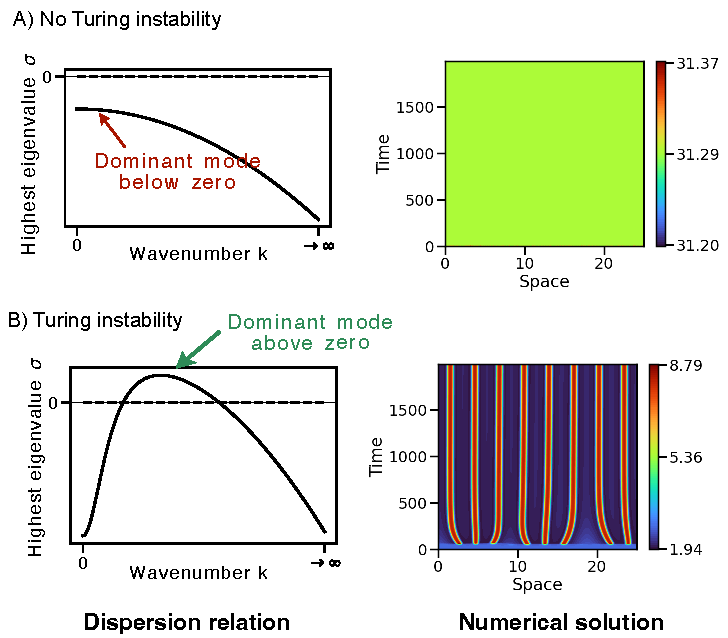
\includegraphics[width=1\textwidth]{chapters/Chapter 1/turing_vs_noturing} % The name of your image file; assumes it's in the same directory as your .tex file
    \caption[\textbf{The turing instability}]{\textbf{The turing instability}}
    \label{fig:turing_vs_noturing} % A label for referencing this figure later in the document
\end{figure}
An example of a classical turing instability with a positive dispersion peak is shown in Fig. \ref{fig:intro_to_turing_patterns}B, along with the corresponding stationary spatial pattern.
Alternatively,  Fig. \ref{fig:turing_vs_noturing}A shows a spatially homogeneous solution which results from a stable system that does not exhibit a diffusion driven instability.
These 1D numerical results were produced using the Crank-Nicholson numerical scheme described in ~\ref{cranknicolson}, which was I programmed from scratch in python. The boundary conditions used are Neumann boundary conditions where the derivative at the boundary is zero ($\pdv{U}{x}=0$) for both molecular species.

%todo add numbers to image
%todo add k and sigma
\subsection{Dataset creation}


\subsection{Infering wavelength and convergence time from dispersion relation}

Although the pattern cannot be observed using linear stability analysis, some information can be obtained from the dispersion relation.
Using the circuit defined in Eq. ~\eqref{eq:turinghill}, we simulated 500 parameter sets with a Turing instabilities as the one seen in Fig. \ref{fig:turing_vs_noturing}B. Then, the convergence time and wavelength for these patterns was measured using the algorithm described in %todo ref methods.
A linear relationship was found between the wavelength in the numerical pattern and the wavelength inferred from the dominant mode of the dispersion relation as seen in Fig. \ref{fig:dispersion_to_wavelength_convergence}A. However, the slope of the regression fitted to the data is smaller than 1, meaning the patterns obtained have a larger wavelength than the predicted linear stability analysis wavelength.
In terms of the convergence time, a non-linear correlation is observed between the highest eigenvalue $(\sigma)$ and the time for convergence.
Although some values do not correlate, we can overall state that systems with high eigenvalues generally converge faster than those lower eigenvalues Fig. \ref{fig:dispersion_to_wavelength_convergence}B.
These relationships are extremely important if we wish to understand characteristics of our system such as wavelength and convergence time without simulating the system numerically.
Specially if scanning through high dimensional spaces, such methods can be extremely informative to get an insight into patterns in this space.
Additionally, these relationships can be used prior to using numerical methods to choose relevant numerical parameters such as length of space and time of our simulation as well as dx and dt.



\begin{figure}[H] % h! is a placement specifier; it tries to place the image here.
    \centering
    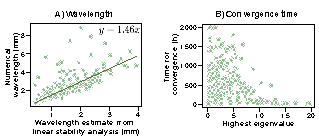
\includegraphics[width=1\textwidth]{chapters/Chapter 1/dispersion_to_wavelength_convergence} % The name of your image file; assumes it's in the same directory as your .tex file
    \caption{A sample caption for the image.}
    \label{fig:dispersion_to_wavelength_convergence} % A label for referencing this figure later in the document
\end{figure}

\subsection{Dispersion to pattern shape}
To further understand the information encoded in the dispersion relation, we focused on the dispersion height.
The approach used consisted in optimizing the dispersion peak height starting from an initial Turing pattern.
This way we can understand what happens to a specific pattern in parameter space when the dispersion peak height increases.
The optimization is carried out using a Markov-Chain Monte Carlo combined with the Metropolis algorithm, where the optimised function is the height of the dispersion peak (e.i the highest value of the highest eigenvalue) (See Methods). %TODO ref methods
The dispersion peak optimization path can be observed in Fig. \ref{fig:dispersion_peak_optimisation}A.
The resulting numerical patterns from the optimisation are then simulated and the convergence time measured as we did for Fig. \ref{fig:dispersion_to_wavelength_convergence}B. In Fig. \ref{fig:dispersion_peak_optimisation}B we can see a cleaner correlation of how the dispersion peak height determines the convergence time which could be modelled with an exponential decay function of the type
\begin{equation}
    f(x) = ae^{bx} + c
\end{equation}

This optimization was carried out for three different initial turing parameter sets. In Fig. \ref{fig:dispersion_peak_optimisation}C we can observe the pattern for the initial turing pattern and the turing pattern after optimization (with the highest dispersion peak).
While the with lower dispersion peaks present labyrinthian type of patterns, the patterns post-optimization present dot-like morphologies.
This suggests that a higher dispersion peak can lead to a preference for spots over labyrinths.


\begin{figure}[H] % h! is a placement specifier; it tries to place the image here.
    \centering
    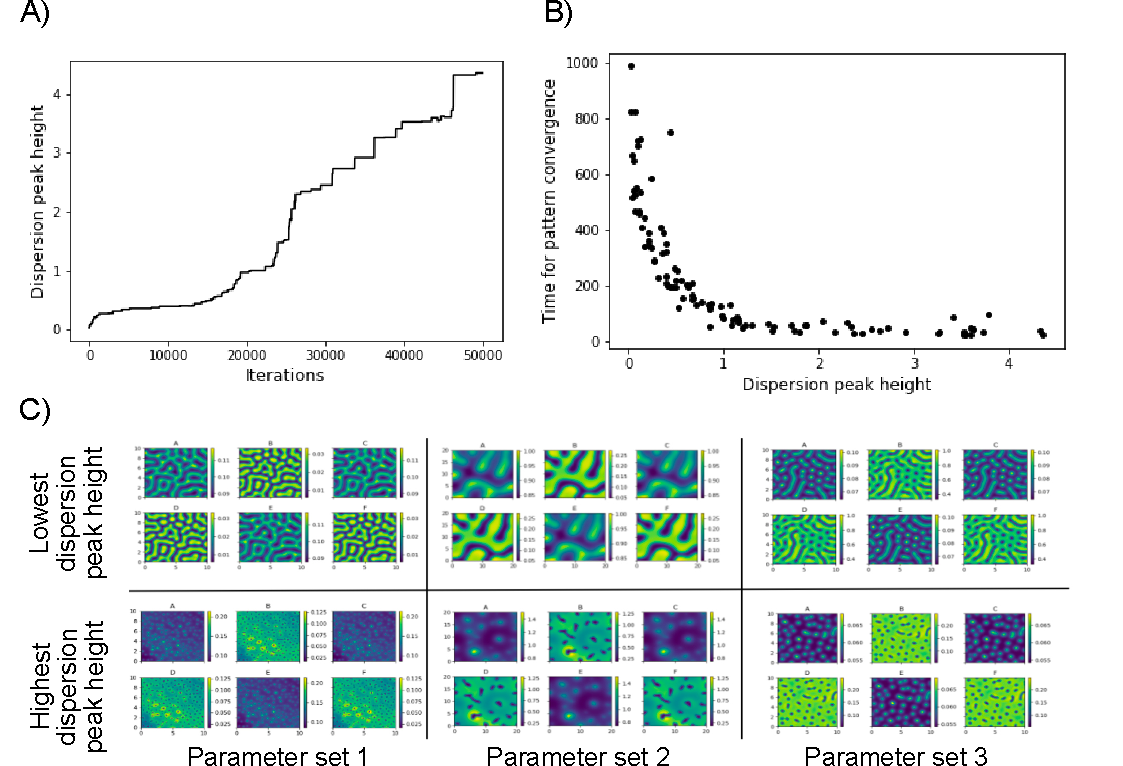
\includegraphics[width=1\textwidth]{chapters/Chapter 1/dispersion_peak_optimisation} % The name of your image file; assumes it's in the same directory as your .tex file
    \caption{A sample caption for the image.}
    \label{fig:dispersion_peak_optimisation} % A label for referencing this figure later in the document
\end{figure}



\section{Breaking linear stability analysis predictions}
Although Turing instabilities are a good indicator of patterned states, these instabilities are neither sufficient nor necessary for stationary periodic patterns to occur.
Current state-of-the-art literature analyses robustness for turing pattern formation using linear stability analysis to determine the Turing patterning parameter space.
With this type of analysis, you have a binary output which determines whether a parameter leads to a classical Turing instability or not as seen in Fig. \ref{fig:lsa_numerical_confusion_literature}.
However, the current assumptions in the TP literature, depicted by this confusion matrix shown in this figure, are a simplification of TPs prediction from linear stability analysis.
This is because the results from linear stability analysis give insights only into the local dynamics around a steady state.
Once the system moves away from the steady state and non-linearities are introduced, the system might behave differently and the local pattern dynamics might not be maintained.
For example, patterning instabilities that are not predicted by linear stability analysis might arise due to a subcritical bifurcations ~\parencite{villar, champneys}.
This is an example of a self-organising pattern where the classical Turing instability conditions are not necessary.


\begin{figure}[H] % h! is a placement specifier; it tries to place the image here.
    \centering
    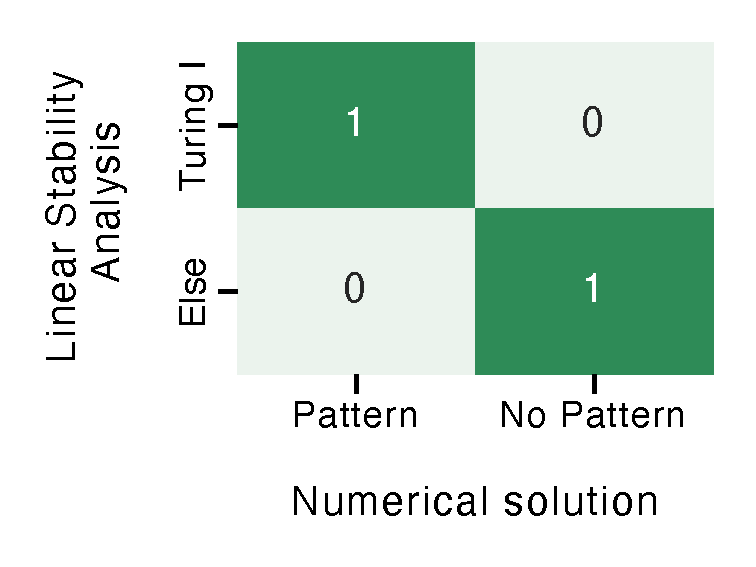
\includegraphics[width=0.6\textwidth]{chapters/Chapter 1/lsa_numerical_confusion_literature} % The name of your image file; assumes it's in the same directory as your .tex file
    \caption{A sample caption for the image.}
    \label{fig:lsa_numerical_confusion_literature} % A label for referencing this figure later in the document
\end{figure}


\subsection{Multistability in Turing}
In this section, we demonstrate how linear-stability is not sufficient or neccesary to predict TPs with multi-stable systems.
The motivation behind this arises from the high degree of multistability exhibited by biological systems, where cell-fate decisions have to be taken within this landscape. %TODO ref scholes thesis (37–40). %todo what leads to multistability? high number of nodes, high cooperativity?
Using the two-node non-linear Turing topology (Eq. \eqref{eq:turinghill}), multi-stable solutions were studied to understand how the patterning dynamics get affected when multiple steady state solutions are found.
First, linear stability analysis is carried out on a particular parameter sets to find multiple steady states of different stability nature (e.g. Stable, Unstable, Turing I, Turing I Hopf).
Then numerical simulations are computed where the initial condition is a random uniform distribution around a particular steady state.
Different pattern outcomes will result depending on where in the phase diagram the initial condition is.
Following the classical hypothesis used in the Turing robustness literature, we would expect Stable and Unstable systems to not produce patterns and Turing to produce patterns.
First, we present how this hypothesis can break under multistability conditions.
Fig. \ref{fig:multistability1} shows a case where diffusion-driven instability conditions are not required for TP formation.
The Unstable system, having a dispersion relation with a peak below zero, managed to get into a TP regime as it is attracted by the Turing equilibrium point.



\begin{figure}[H] % h! is a placement specifier; it tries to place the image here.
    \centering
    \begin{adjustbox}{center}
        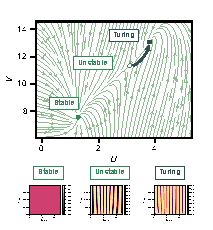
\includegraphics[width=1\textwidth]{chapters/Chapter 1/multistability1} % The name of your image file; assumes it's in the same directory as your .tex file
    \end{adjustbox}
    \caption{Turing pattern regimes attract neighbouring non-patterning equilibrium states.}
    \label{fig:multistability1} % A label for referencing this figure later in the document
\end{figure}

Then, we present a case where linear stability analysis cannot predict TP formation. Fig.~\ref{fig:multistability2} shows an ephemeral or transient pattern that occurs in the Unstable and Turing regimes.
The TP initially develops in the vicinity of the Turing steady state.
As the spatial heterogeneity is amplified and settles, it gets attracted by the stable steady state leading to the disruption of the pattern.
This type of transient pattern behaviour has also been recently reported in ~\cite{Krause2023}.

\begin{figure}[H] % h! is a placement specifier; it tries to place the image here.
    \centering
    \begin{adjustbox}{center}
        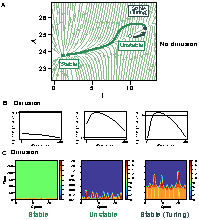
\includegraphics[width=1\textwidth]{chapters/Chapter 1/multistability2} % The name of your image file; assumes it's in the same directory as your .tex file
    \end{adjustbox}
    \caption{Ephemeral patterns}
    \label{fig:multistability2} % A label for referencing this figure later in the document
\end{figure}

Other examples can also be found, for example, where the unstable system settles into Turing, but the Turing system gets pulled by the Stable attractor (Fig.~\ref{fig:multistability_leftover}A). Additionally, some systems don't even exhibit a transient pattern and the three solutions are homogeneous in time and space (Fig.~\ref{fig:multistability_leftover}B). Finally, an unstable point might lie between to Turing points and therefore all three solutions will be a stationary periodic pattern (Fig.~\ref{fig:multistability_leftover}C).


\begin{figure}[H] % h! is a placement specifier; it tries to place the image here.
    \centering
    \begin{adjustbox}{center}
    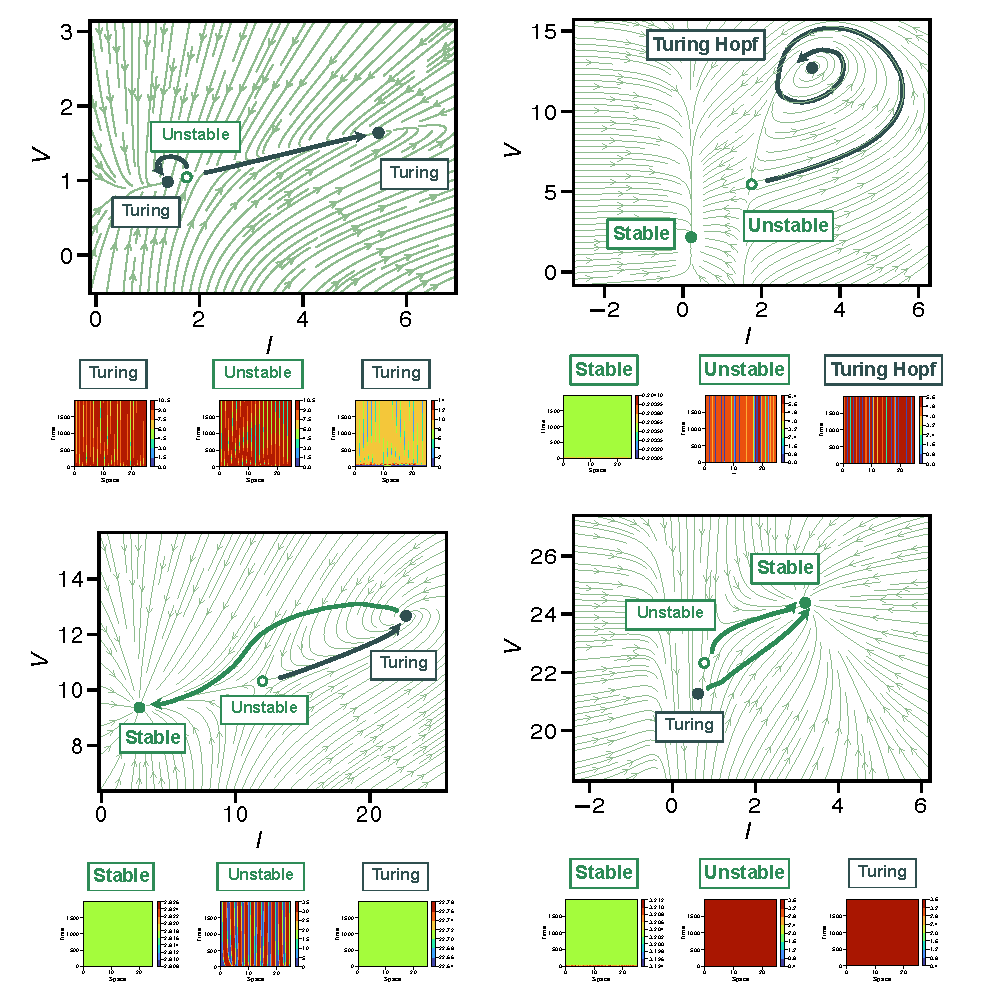
\includegraphics[width=1.4\textwidth]{chapters/Chapter 1/multistability_leftover} % The name of your image file; assumes it's in the same directory as your .tex file
    \end{adjustbox}
    \caption{Other types of multistability regimes.}
    \label{fig:multistability_leftover} % A label for referencing this figure later in the document
%TODO make subfigures bigger. Add letters to subfigures
\end{figure}


\subsection{Analytical to numerical: Other types of dispersion relation, and other types of patterns}
Multi-stable systems are not the only case where the classical turing instability fails to predict pattern formation.
Other types of dispersion relation beyond classical Turing instabilities can produce stationary patterns and non-stationary regular patterns that might be of interest in developmental biology.
The aim of this section is to document what type of dispersion relations in mono-stable systems can be linked to what type of patterns to gain insights into predicting pattern formation from linear stability analysis.
We will first present a classification for the different types of dispersion relation.
Then we will show the classification for the different types of pattern outcomes.
Finally, we will reconstruct the 2x2 confusion matrix (Fig. ~\ref{fig:lsa_numerical_confusion_literature}) currently used as an assumption in the literature for pattern formation to show a more complete understanding. The new confusion matrix will show more types of dispersion relation and more pattern outcomes with leading to a 5x4 confusion matrix.

First, we classify the outputs of dispersion relations from linear stability analysis into 5 types.
Stable dispersion relations have all eigenvalues $\sigma$ below zero for any wavenumber $k$, meaning there is no instability (Fig ~\ref{fig:dispersions}A).
Unstable dispersion relations have a positive eigenvalue at $k=0$ which eventually drops below zero as diffusion is introduced $k>0$ (Fig ~\ref{fig:dispersions}B).
As the unstable dispersion relation, the Hopf dispersion relation occurs when there is an instability without diffusion ($\sigma>0$ for $k=0$) which eventually drops below zero for positive wavenumbers.
However, in the case of Hopf dispersion relation, when the eigenvalues cross the zero line, there is a pair of complex conjugate eigenvalues (Fig ~\ref{fig:dispersions}C).
Turing I dispersion relations, as previously mentioned, are stable without diffusion and have an instability for a positive wavenumber and finally stable again for very large wavenumbers (Fig ~\ref{fig:dispersions}D).
Finally, Turing I hopf dispersion relations, are a combination of Turing I and Hopf dispersion relations.
As the Hopf bifurcation, they are unstable without diffusion.
Then, the stability kicks in with a pair of complex conjugates as the eigenvalues cross the zero line.
Finally, a Turing I type behaviour kicks in getting a peak above zero and decaying again for large wavenumbers (Fig ~\ref{fig:dispersions}E).
Other types of dispersion relation exist which are not displayed here such as Turing II, where the eigenvalues do not become stable again for very large wavenumbers.
Therefore, this system displays an instability at very large wavenumbers which result in infinitesimally small wavelength patterns.
These are considered to produce homogeneous solutions, except in the case of space discretization where they can produce small wavelength patterns ~\parencite{Wang2022}.
%TODO More detail on this classification can be found in methods x



%todo . They also identify examples of non-stationary spatial patterns, when the eigenvalue corresponding to a critical wave number has non-zero imaginary part.Deutsch, A., Dormann, S., et al., 2005. Cellular automaton modeling of biological pattern formation. Springer.

%todo look at pitchfork and transcritical

\begin{figure}[H] % h! is a placement specifier; it tries to place the image here.
    \centering
    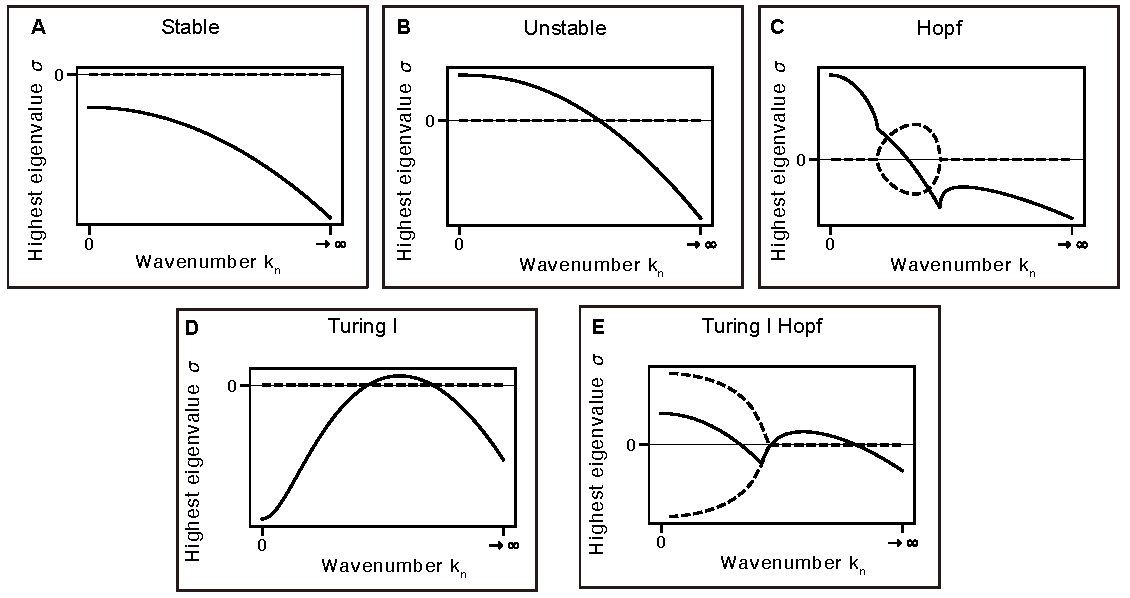
\includegraphics[width=1\textwidth]{chapters/Chapter 1/dispersions} % The name of your image file; assumes it's in the same directory as your .tex file
    \caption{A sample caption for the image.}
    \label{fig:dispersions} % A label for referencing this figure later in the document
\end{figure} %TODO add k and sigma to plots

We then need to classify the different types of patterns outcomes into 4.
We use a decision tree for the classification where the two layers are spatial homogeneity and convergence in time, as seen in Fig. ~\ref{fig:no growth classification}.
A pattern will be considered homogeneous if the final snapshot $U$ for any of the two molecular species fulfills the following condition
\begin{equation}
    \frac{max(U) - min(U)}{max(U)} \leq 0.01
\end{equation}
A pattern will be considered converged if the last 30 timepoints for any of the two molecular species fulfills the following condition
\begin{equation}
    \frac{max(U[-30:]) - min(U[-30:])}{max(U[-30:])} \leq 0.05
\end{equation}
The thresholds chosen were fine-tuned by testing them on the numerical patterns to obtain the best classification results.
Using this two characteristics, homogeneity and convergence, we can obtain 4 classes of patterns: Homogeneous, Temporal Oscillators, Non-stationary Patterns and Stationary Patterns (See Fig. ~\ref{fig:no growth classification}).
Homogeneous patterns are homogeneous in space and converge in time.
Temporal oscillators are homogeneous in space but do not converge, as they oscillate in time.
Non-stationary patterns are not homogeneous in space and do not converge in time.
Instead they show a spatial pattern that changes over time.
Finally, Stationary patterns are not homogeneous in pace but converge in time.


\begin{figure}[H] % h! is a placement specifier; it tries to place the image here.
    \centering
    \begin{adjustbox}{center}
    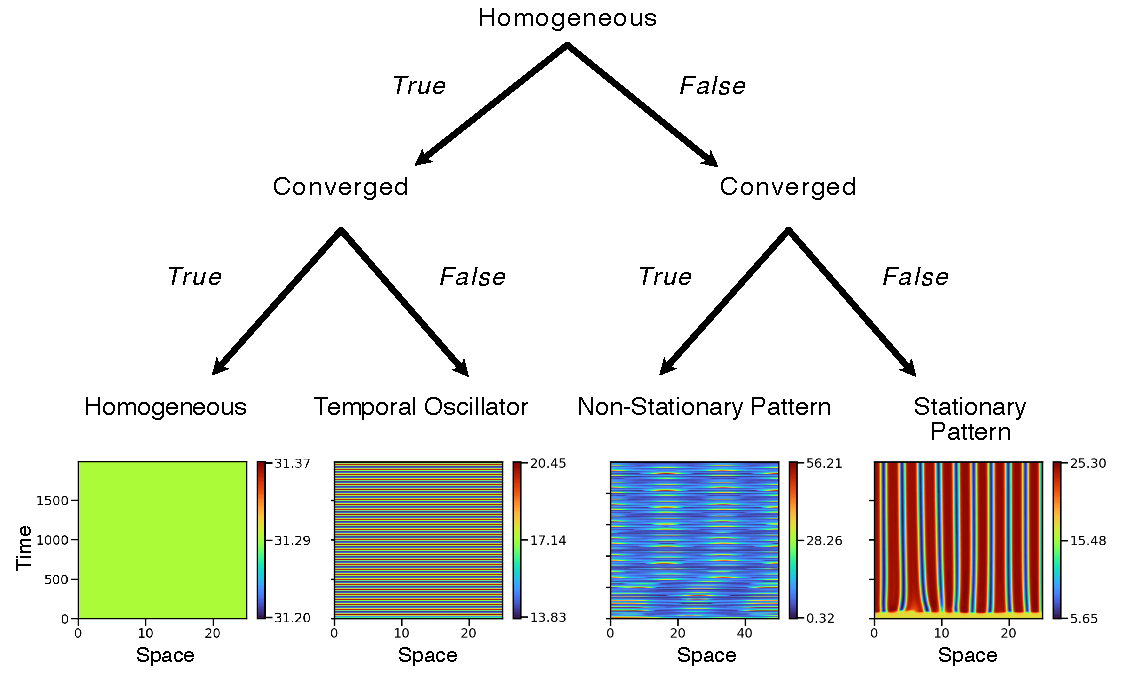
\includegraphics[width=1.2\textwidth]{chapters/Chapter 1/no growth classification} % The name of your image file; assumes it's in the same directory as your .tex file
    \end{adjustbox}
    \caption{Decision tree to classify patterns in non-growing domains}
    \label{fig:no growth classification} % A label for referencing this figure later in the document
\end{figure}


High throughput studies like ~\cite{Scholes2019, Zheng2016, Marcon} only consider Turing I as patterning and the rest is discarded.
Here, we explore beyond turing I and stationary patterns to give a more complete view of the relationship between linear stability and spatio-temporal patterns.
10000 parameter sets are analysed from the non-linear turing model (Eqs. \eqref{eq:turinghill}) to obtain dispersions relation numerical patterns.
Multi-stable systems are not included in this analysis to understand the direct relationships between the dispersion relation and numerics.
The two types of classifications describe above are applied, and a new 5x4 confusion matrix is generated (Fig. ~\ref{fig:lsa_numerical_confusion}).  %TODO check number of params

\begin{figure}[H] % h! is a placement specifier; it tries to place the image here.
    \centering
    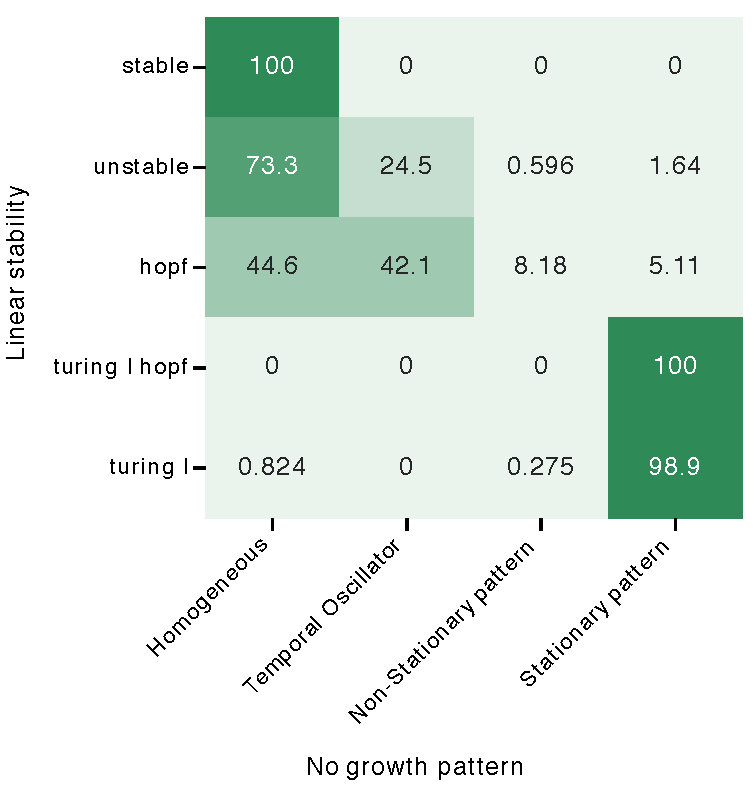
\includegraphics[width=1\textwidth]{chapters/Chapter 1/lsa_numerical_confusion} % The name of your image file; assumes it's in the same directory as your .tex file
    \caption{\textbf{Confusion matrix to relate Linear stability Analysis output and numerical pattern outcome}}
    \label{fig:lsa_numerical_confusion} % A label for referencing this figure later in the document
\end{figure}

It is worth pointing out some interesting examples obtained from this confusion matrix.
For example, Turing I hopf seems to always lead to stationary patterns (See Fig. \ref{fig:interesting_cases_nogrowth}B), meaning they would definitely need to be included in high throughput robustness studies.
Some unstable dispersion relations lead to both stationary (See Fig. \ref{fig:interesting_cases_nogrowth}A) and non-stationary patterns.
Additionally, Hopf solutions also display interesting non-stationary patterns (See Fig. \ref{fig:interesting_cases_nogrowth}D).
Non-stationary patterns could also be of big interest in the field of developmental and synthetic biology as gene expression arrest could turn them into periodic stationary patterns.
Additionally, these non-stationary patterns could serve as a periodic pre-pattern for the initial symmetry breaking.
Unfortunately, some Hopf solutions are misclassified as Stationary patterns (See Fig. \ref{fig:interesting_cases_nogrowth}C) due to an inadequate threshold in the convergence classification.
It is important to understand that this is an initial exploratory analysis where classification might occur. This is because of the difficulty of common setting thresholds for a wide variety of numerica solutions with different wavelengths, time-scales and dynamic ranges.

\begin{figure}[H] % h! is a placement specifier; it tries to place the image here.
    \centering
    \begin{adjustbox}{center}
        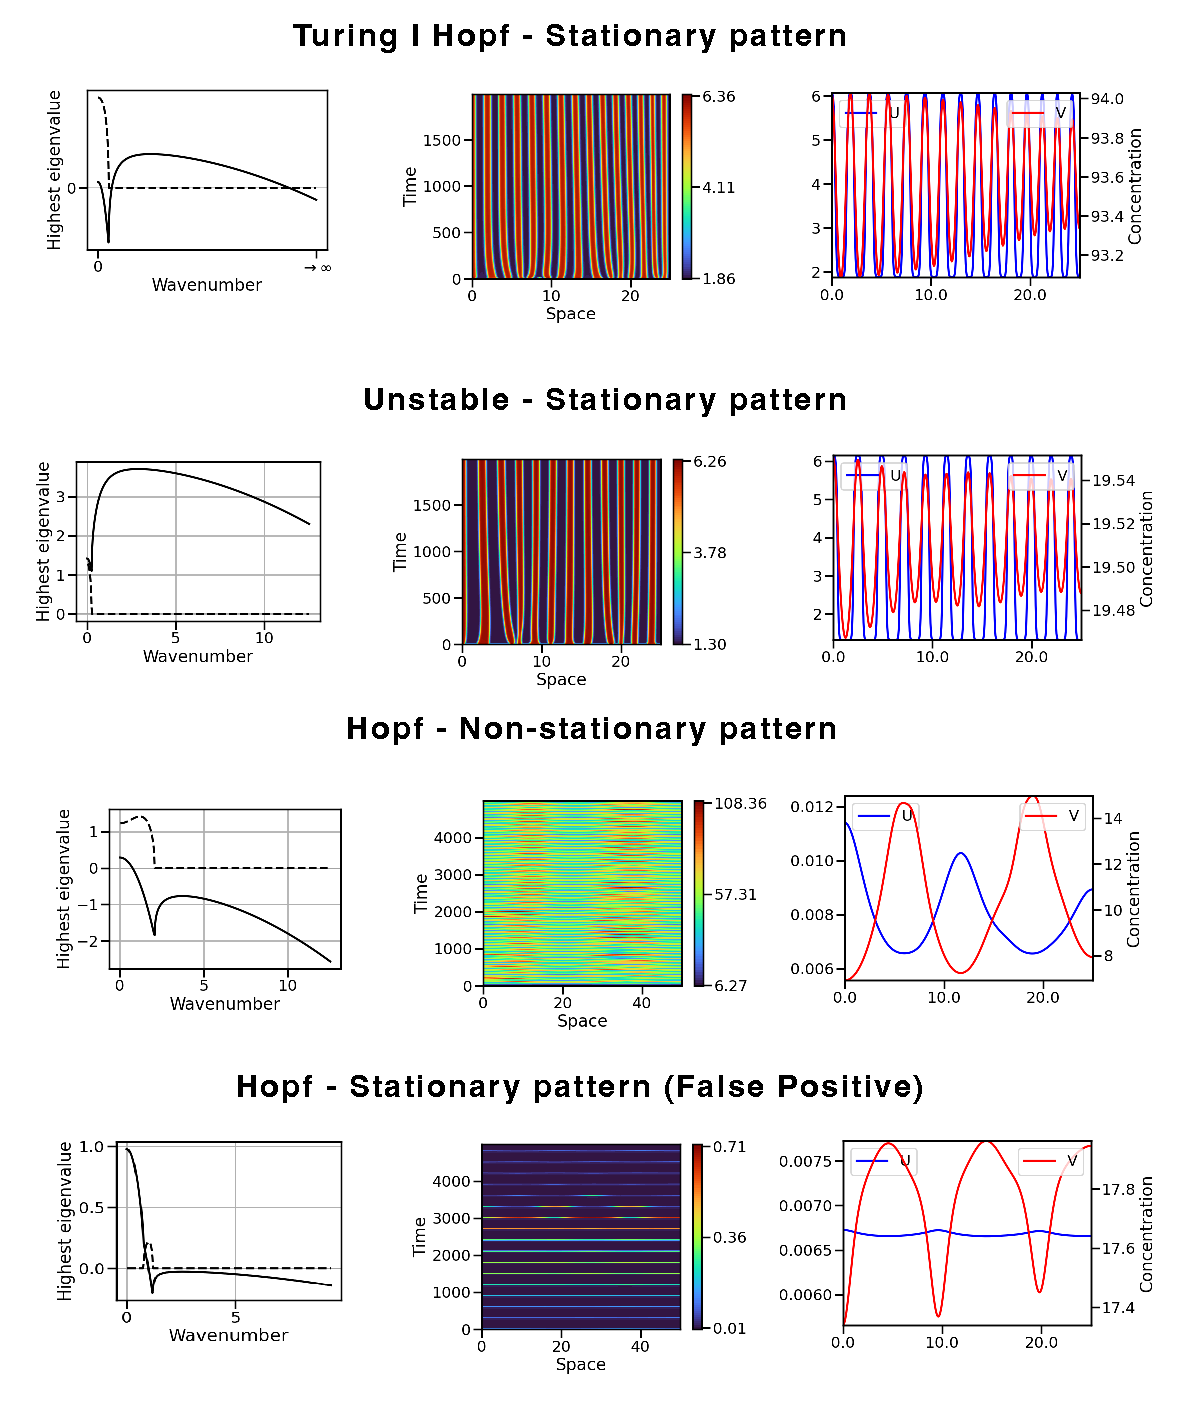
\includegraphics[width=1.2\textwidth]{chapters/Chapter 1/interesting_cases_nogrowth} % The name of your image file; assumes it's in the same directory as your .tex file
    \end{adjustbox}
    \caption{Interesting examples obtained from confusion matrix. }
    \label{fig:interesting_cases_nogrowth} % A label for referencing this figure later in the document
\end{figure}
\section{Introducing realistic biological phenomena}
As seen in the previous section both multistability effects and numerical solutions can break the hypothesis that only classical Turing I systems can produce stationary periodic patterns.
Here, we look deeper into how other aspects linking the theory closer to the biological reality can also break this hypothesis.
In particular, we will look at how adding an absorbing boundary condition and growth to the Turing problem might induce or break patterning.
This particular direction was inspired in experiments described in the next sections where growing bacterial colonies are used as a platform to engineer Turing patterns using synthetic gene circuits.

The absorbing boundaries are introduced by using a Dirilichet boundary condition where the concentration at the boundary is zero $u=0$ as opposed to the previously used Neumann boundaries where the derivative at the boundary is zero.
On the other hand, growth is introduced as isotropic linear growth, where cells are added to both boundaries with a linear growth rate.
Growth of the tissue is encoded in a 1D binary vector, where cells are denoted as 1 and empty space as 0.
The amount of 1's grows linearly, which represents the tissue expanding.
This vector is used as a mask, where 1's determine the computation of reaction-diffusion terms and 0's determine only the computation of diffusion.
Therefore, while reaction-diffusion occurs in the tissue; only diffusion occurs in the empty regions.

As with the non-growing Neumann boundary condition patterns in the previous section, we develop a classification system to quantify the different types of patterns obtained, and the transitions as growth is introduced.
However, due to the absorbing boundary conditions and growth homogeneity and convergence we previously defined is in some cases physically impossible.
For this reason, a new classification system is developed based on the number of peaks.
Peaks are detected using the python $find\_peaks$ algorithm with parameter
$prominence=0.05$.
Again, this can be tweeked depending on the numerical outcome and misclassification might occur.


\begin{figure}[H] % h! is a placement specifier; it tries to place the image here.
    \centering
    \begin{adjustbox}{center}
        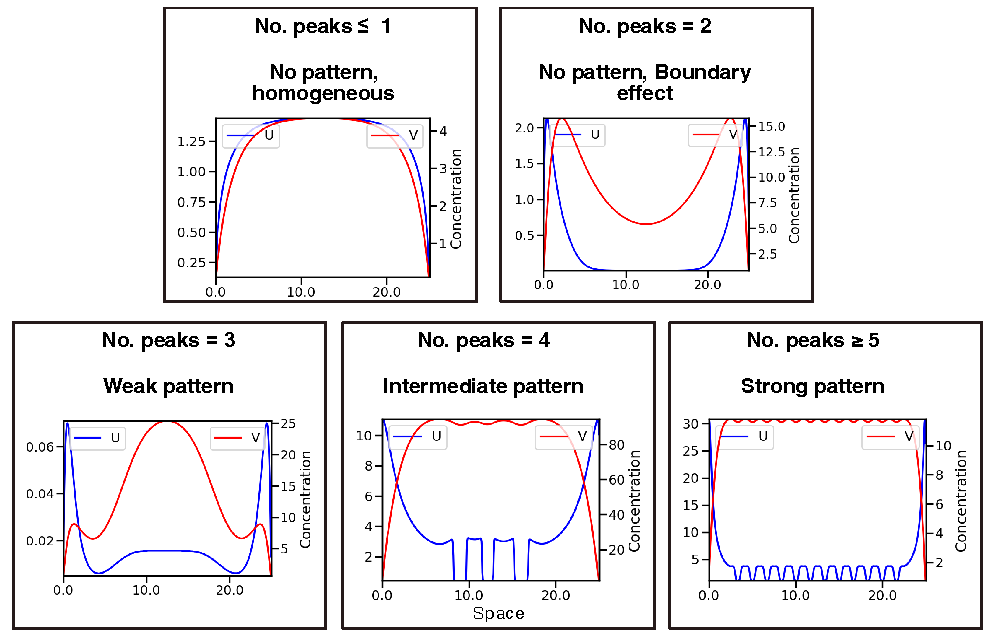
\includegraphics[width=1\textwidth]{chapters/Chapter 1/peaks_classification} % The name of your image file; assumes it's in the same directory as your .tex file
    \end{adjustbox}
    \caption{Classification based on peaks for absorbing boundary conditions and growth}
    \label{fig:peaks_classification} % A label for referencing this figure later in the document
\end{figure}

The peak classification shown in \ref{fig:peaks_classification}, retrieves information on whether there is a pattern at all and whether this pattern is only a pattern at the boundary or is a periodic pattern due to other effects.
Patterns with one 1 peak will be considered homogeneous as they result from the morphogens being reduced at the boundary due to absorption.
Patterns with 2 peaks are also considered not to be patterned states as the two peaks might arise at the boundary for one of the diffusers due to the depletion of the other.
Patterns with 3 peaks start displaying a more significant pattern, although it is hard to prove periodicity from them and the number of peaks might not scale with tissue length.
Patterns with 4 peaks could still be purely a boundary effect, but is less likely as periodicity starts being more present.
Finally, patterns with 5 peaks and above can be considered strong patterns and would be most similar to classical Turing patterns in non-growing no-flux boundary domains.


Using this classification method, x parameter sets where simulated and classified with absorbing boundary conditions and growth
%TODO make image on classification
%TODO add  2 confusion matrix


\subsection{No growth to open boundaries}

\begin{figure}[H] % h! is a placement specifier; it tries to place the image here.
    \centering
    \begin{adjustbox}{center}
        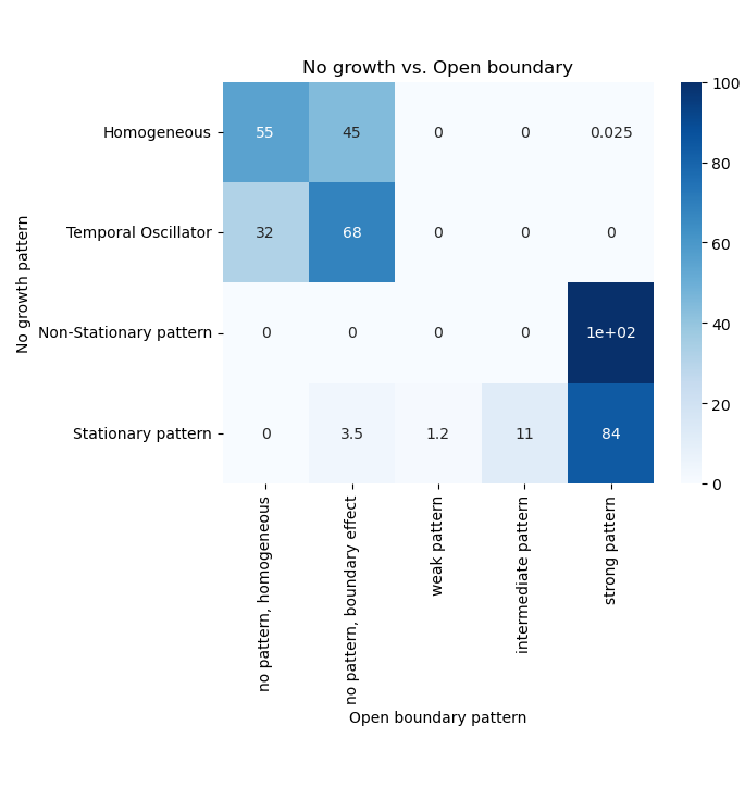
\includegraphics[width=1\textwidth]{chapters/Chapter 1/nogrowth_openboundary} % The name of your image file; assumes it's in the same directory as your .tex file
    \end{adjustbox}
    \caption{Classification based on peaks for absorbing boundary conditions and growth}
    \label{fig:nogrowth_openboundary} % A label for referencing this figure later in the document
\end{figure}


\subsection{Open boundaries to growth}

\begin{figure}[H] % h! is a placement specifier; it tries to place the image here.
    \centering
    \begin{adjustbox}{center}
        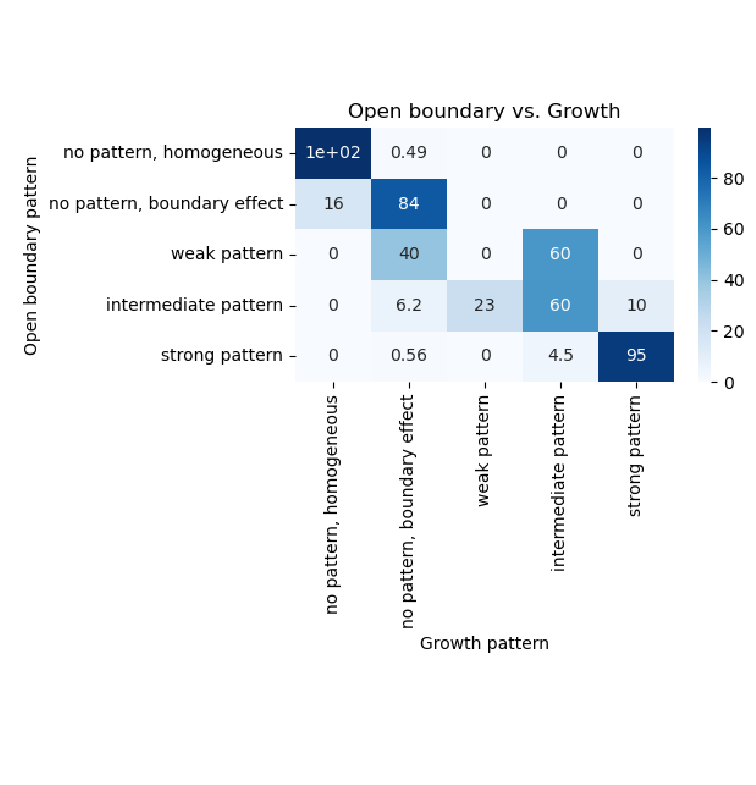
\includegraphics[width=1\textwidth]{chapters/Chapter 1/openboundary_edgegrowth2} % The name of your image file; assumes it's in the same directory as your .tex file
    \end{adjustbox}
    \caption{Classification based on peaks for absorbing boundary conditions and growth}
    \label{fig:openboundary_edgegrowth2} % A label for referencing this figure later in the document
\end{figure}





\begin{figure}[H] % h! is a placement specifier; it tries to place the image here.
    \centering
    \begin{adjustbox}{center}
        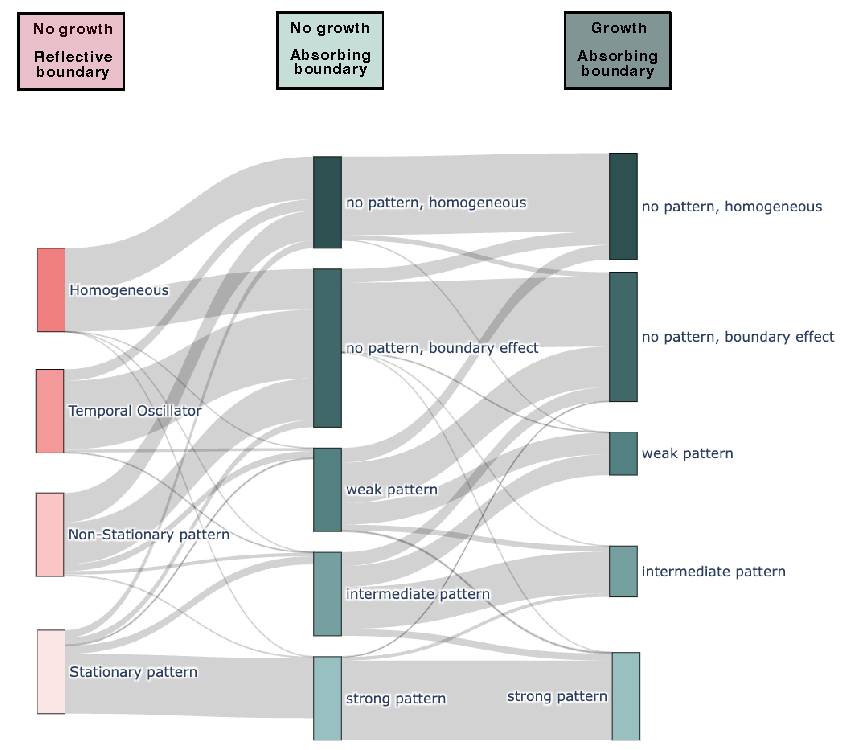
\includegraphics[width=1\textwidth]{chapters/Chapter 1/3layer_sankey} % The name of your image file; assumes it's in the same directory as your .tex file
    \end{adjustbox}
    \caption{Classification based on peaks for absorbing boundary conditions and growth}
    \label{fig:3layer_sankey} % A label for referencing this figure later in the document
\end{figure}







